\chapter{Gestione della concorrenza}
Per i sistemi operativi moderni è essenziale supportare più processi in esecuzione. In tal senso un grosso problema da affrontare è la \textit{concorrenza}, ovvero la gestione del modo con qui questi processi interagiscono. In generale la concorrenza si manifesta quando ci sono delle applicazioni multiple che condividono il tempo di calcolo, quando ci sono delle applicazioni strutturate per essere parallele, oppure semplicemente quando il sistema operativo stesso ha più processi o thread in esecuzione.

\subsection*{Race condition}
Una \textit{sezione critica} è una parte di un processo in cui avviene un accesso ad una risorsa condivisa. Con la \textit{mutua esclusione} si cerca di imporre che solo un processo possa accedere alla sezione critica e quindi si vuole evitare: \textit{race condition} violazione della mutua esclusione; \textit{deadlock} o stallo, quando duo o più processi non possono procedere nell'esecuzione perché ciascuno attende l'altro; \textit{livelock} o stallo attivo, quando due o più processi cambiano continuamente il proprio stato; \textit{starvation} o morte per fame, quando un processo non viene mai scelto dallo scheduler.

La difficoltà principale con la concorrenza è che non si può fare nessuna assunzione o previsione sul comportamento dei processi e sullo scheduler.

\begin{Example}{Risorse condivise}{}
   \textit{Dato il seguente pseudocodice di una funzione che prende un valore in input e lo scrive in output:}
    \begin{verbatim}
        void echo()
        {
            chin = getchar();
            chout = chin;
            putchar(chout);
        }
    \end{verbatim}
    \textit{supponiamo che due processi $P_1$ e $P_2$ cercano di eseguire questo codice su un processore.}
    \begin{verbatim}
        Process P1              Process P2
              .                       .
        chin = getchar();             .
              .                 chin = getchar();
        chout = chin;                 .
              .                 chout = chin;
        putchar(chout);               .
              .                 putchar(chout);
              .                       .
    \end{verbatim}
    Notiamo come \verb|chin| viene sovrascritto dal processo $P_2$ generando problemi di race condition su risorse condivise. Il problema si può risolvere facendo sì che la funzione \verb|echo| possa essere eseguita solo da un processo alla volta.
\end{Example}

Il sistema operativo si deve assicurare che processi ed output siano indipendenti dalla velocità di computazione (ovvero dallo scheduling), quindi quando un processo ha la necessità di accedere alle risorse deve fare una richiesta al sistema operativo (tramite syscall). Tuttavia, non è sempre possibile, ad esempio se occorre accedere ad una risorsa che potrebbe essere condivisa con altri processi, occorre fare una richiesta di bloccaggio della risorsa. Quindi gli stessi processi devono essere scritti pensando già alla cooperazione, usando opportune syscall (es. semafori) e scrivendo le funzioni di \verb|entercritical| e \verb|exitcritical|.

\subsection*{Requisiti per la mutua esclusione}
Qualsiasi meccanismo si usi per offrire la mutua esclusione, deve soddisfare i seguenti requisiti: solo un processo alla volta può essere nella sezione critica per una risorsa; non si deve generare deadlock o starvation; un processo deve entrare subito nella sezione critica se nessun altro processo usa la risorsa; un processo che si trova nella sua sezione non-critica non deve subire interferenza da altri processi; un processo che si trova nella sezione critica ne deve prima o poi uscire.

\section{Mutua esclusione: supporto hardware}
Una prima idea per effettuare la mutua esclusione è disabilitare gli interrupt prima di entrare nella sezione critica per poi abilitarli una volta usciti. Disabilitare le interruzioni garantisce la mutua esclusione ovvero, se il processo può decidere di non essere interrotto, allora nessun altro lo può interromperlo mentre si trova nella
sezione critica, ma non funziona su sistemi con più processori e se i processi ne abusano peggiorano le prestazioni del sistema operativo.

Un'altra opzione è utilizzare delle istruzioni macchina speciali:
\begin{lstlisting}[language=C]
    int compare_and_swap(int word, int testval, int newval)
    {
        int oldval;
        oldval = word;
        if (word == testval) word = newval;
        return oldval
    }

    void exchange(int register, int memory)
    {
        int temp;
        temp = memory;
        memory = register;
        register = temp;
    }
\end{lstlisting}

L'hardware garantisce che un solo processo per volta possa eseguire una chiamata a tali funzioni anche se ci sono più processori (vedi Figura \ref{fig:mutua-esclusione-istruzioni}).

\begin{figure}[h]
    \centering
    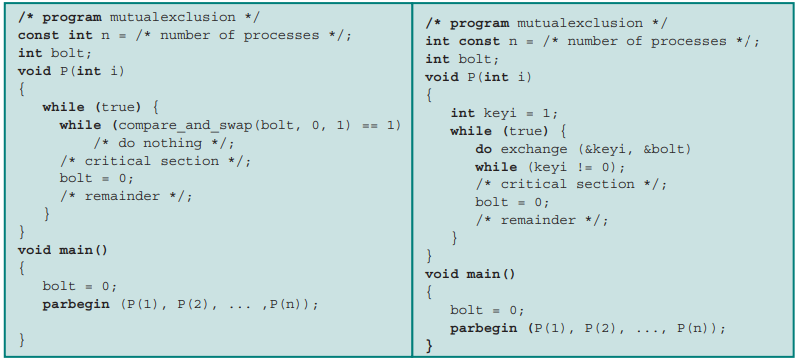
\includegraphics[width=1\linewidth]{images/mutua-esclusione-istruzioni.PNG}
    \caption{Mutua esclusione con compare\_and\_swap e exchange}
    \label{fig:mutua-esclusione-istruzioni}
\end{figure}

In entrambi i casi l'idea è che il processo che trova bolt a 0 può eseguire la \verb|critical section| e, per impedire ad altri di entrare, mette bolt a 1. Una volta terminato, rimette bolt a 0, così gli altri processi possono accedere alla sezione o anche lui stesso, se è solo oppure se lo scheduler lo favorisce.

Questo tipo di approccio è applicabile a qualsiasi numero di processi, sia su un sistema ad
un solo processore che ad un sistema a più processori con memoria condivisa e possono essere usate per gestire sezioni critiche multiple. Ma è anche vero che si possono generare \textit{busy-waiting} (spreco di tempo di computazione), starvation e deadlock.

Per superare tutti questi ostacoli possiamo utlizzare i semafori.

\section{Semafori}
Un \textit{semaforo} è una particolare struttura dati sulla quale è possibile fare solo tre operazioni atomiche con il supporto di un valore intero utilizzato per scambiare segnali con i processi. Queste operazioni sono: \verb|initialize|, \verb|decrement| o \verb|semWait| che può mettere il processo in blocked, \verb|increment| o \verb|semSignal| che può mettere un processo blocked in ready. Si tratta di syscall che sono eseguite in kernel mode e possono agire direttamente sui processi.

\begin{lstlisting}[language=C]
    struct semaphore {
        int count;
        queueType queue;
    };
    void semWait(semaphore s)
    {
         s.count--;
         if (s.count < 0) {
             /* place this process in s.queue */;
             /* block this process */;
         }
    }
    void semSignal(semaphore s)
    {
         s.count++;
         if (s.count<= 0) {
             /* remove a process P from s.queue */;
             /* place process P on ready list */;
         }
    }
\end{lstlisting}
\vspace{-0.5cm}\captionof{lstlisting}{Definizione di un semaforo}\vspace{0.5cm}

Il sistema operativo usa una coda per memorizzare i processi in attesa su un semaforo, ma quale politica viene usata per prendere il prossimo processo in attesa nella coda? Se si usa la FIFO, allora si parla di \textit{strong semaphore} (semaforo forte); se la politica non viene specificata, allora si parla di \textit{weak semaphore} (semaforo debole).

\begin{Example}{Funzionamento di un semaforo}{}
    \textit{Supponiamo di avere un semaforo $s$ con il suo valore intero e la sua coda di processi.} 
    
    \circled{1} dal dispatcher viene scelto il processo $A$ per andare in esecuzione e viene invocata la funzione \verb|semWait| in modo da \circled{2} inserire $A$ nella coda e mandare in esecuzione il processo $B$. Ora se viene invocata una \verb|semWait| il valore del semaforo viene decrementato a -1 e \circled{3} il processo $B$ finisce nella coda dei blocked. \circled{4} nel momento in cui viene eseguito $D$ si effettua una \verb|semSignal| e il processo $B$ torna nella corda dei Ready. \circled{5} ora è in esecuzione il processo $C$ e vengono eseguite tre \verb|semWait|, \circled{6} quindi il valore intero passa a -3 e nella coda dei blocked ci sono i processi $B, A, C$. \circled{7} quando verrà eseguita una \verb|semSignal| un semaforo forte sblocca il primo processo della coda e lo inserisce nei Ready.

    \begin{minipage}{\textwidth}
        \centering
        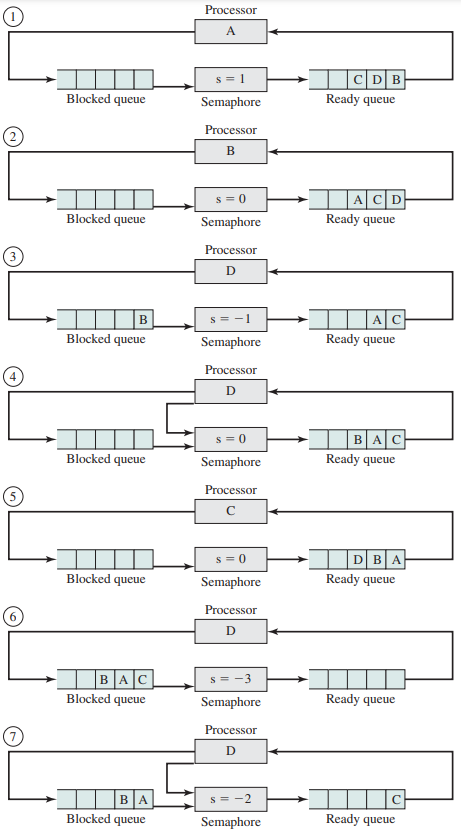
\includegraphics[width=0.49\linewidth]{images/esempio-semaforo.PNG}
        %\captionof{figure}{Esempio di semaforo}
    \end{minipage}
\end{Example}

\begin{figure}[h]
    \centering
    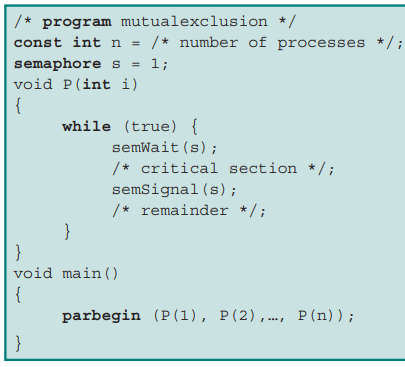
\includegraphics[width=0.5\linewidth]{images/mutua-esclusione-semafori.PNG}
    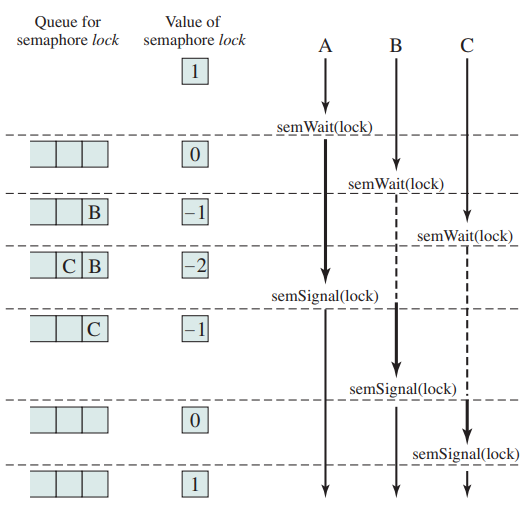
\includegraphics[width=0.49\linewidth]{images/mutua-esclusione-semafori2.PNG}
    \caption{Mutua esclusione con i semafori}
    \label{fig:mutua-esclusione-semafori}
\end{figure}

\subsection*{Problema dal produttore/consumatore}
Ci sono uno o più processi produttori che creano dati e li mettono in un buffer, un consumatore prende dati dal buffer uno alla volta e al buffer può accedere un solo processo, sia esso produttore o consumatore. Il problema nasce quando si vuole assicurare che i produttori non inseriscano dati quando il buffer è pieno e che il consumatore non prenda dati quando il buffer è vuoto.

Ipotizzando di avere un buffer infinito possiamo scrivere il codice del produttore e consumatore come segue:
\begin{lstlisting}[language=C]
    while(true) {
        /* produce item v */
        b[in] = v;
        in++;
    }

    while(true) {
        while(in <= out)
            /* do nothing */;
        w = b[out];
        out++;
        /* consume item w */
    }
\end{lstlisting}

La corretta soluzione per risolvere i problemi visti è in Figura \ref{fig:soluzione-buffer}.
\begin{figure}[h]
    \centering
    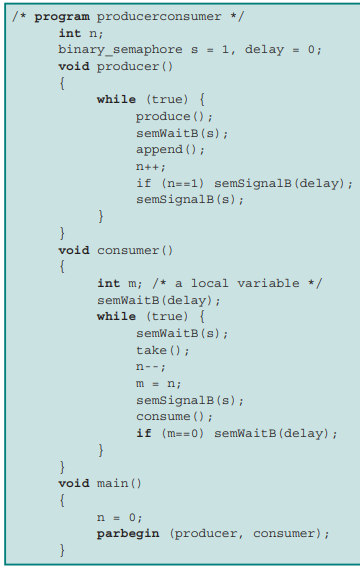
\includegraphics[width=0.49\linewidth]{images/soluzione-buffer.PNG}
    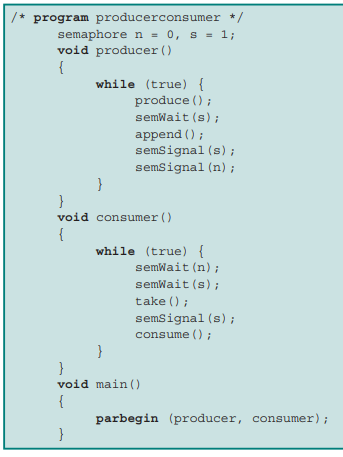
\includegraphics[width=0.5\linewidth]{images/soluzione-buffer2.PNG}
    \caption{Soluzione del produttore/consumatore con semafori binari e generali}
    \label{fig:soluzione-buffer}
\end{figure}

\subsection*{Implementazione dei semafori}
La vera implementazione dei semafori è con buffer finiti e circolari. Anche con questo tipo di semafori ci sono due puntatori \verb|In| e \verb|Out| grazie ai quali i produttori/consumatori svolgono le loro operazioni.

\begin{figure}[h]
    \centering
    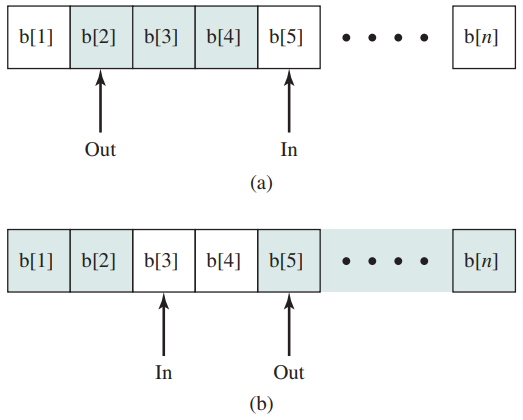
\includegraphics[width=0.5\linewidth]{images/semafori-circolari.PNG}
    \caption{Buffer circolare finito}
    \label{fig:semafori-circolari}
\end{figure}

La dimensione effettiva del buffer è $n - 1$, altrimenti non si potrebbe capire se $in == out$ implichi buffer pieno o vuoto. I codici del produttore e consumatore diventano:
\begin{lstlisting}[language=C]
    while(true) {
        /* produce item v */
        while((in + 1) % n == out)
            /* do nothing */;
        b[in] = v;
        in = (in + 1) % n;
    }

    while(true) {
        while(in == out)
            /* do nothing */;
        w = b[out];
        out = (out + 1) % n;
        /* consume item w */
    }
\end{lstlisting}

\begin{figure}[h]
    \centering
    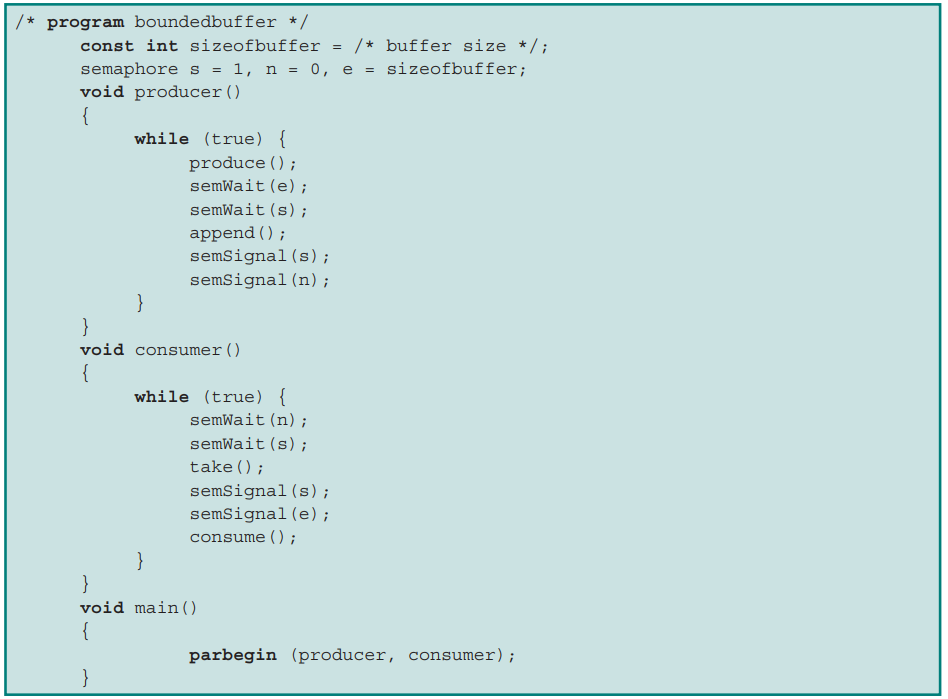
\includegraphics[width=1\linewidth]{images/prod-cons-buffer-circ.PNG}
    \caption{Produttori e consumatori con buffer circolari}
    \label{fig:prod-cons-buffer-circ}
\end{figure}

\begin{Example}{Trastevere}{}
    \textit{Supponiamo di voler risolvere il seguente problema: sulla strada di Trastevere a doppio senso, per un breve tratto, la strada si restringe e diventa a senso unico alternato con al massimo quattro macchine di passaggio. Una volta impegnata da un lato, tutte le macchine dall'altro lato devono aspettare che non ci siano più macchine né sulla strettoia, né in coda. Scrivere una funzione che gestisca il comportamento delle macchine di sinistra e di destra.}

    \begin{minipage}{\textwidth}
        \centering
        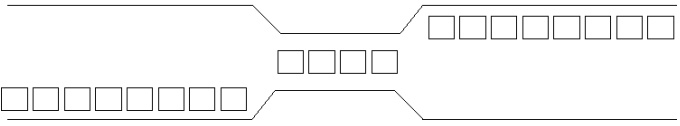
\includegraphics[width=0.7\linewidth]{images/trastevere.PNG}
        %\captionof{figure}{Esempio di semaforo}
    \end{minipage}

    La funzione rischiesta è la seguente:
    \begin{lstlisting}[language=C]
    semaphore z = 1;
    semaphore strettoia = 4;
    semaphore sx = 1;
    semaphore dx = 1;
    int nsx = 0;
    int ndx = 0;
    
    macchina_dal_lato_sinistro () {
        wait(z);
        wait(sx) ;
        ++nsx;
        if(nsx == 1)
            wait(dx);
        signal(sx);
        signal(z);
        wait(strettoia);
        passa_strettoia();
        signal(strettoia);
        wait(sx);
        --nsx;
        if(nsx == 0)
            signal(dx);
        signal(sx);
    }
    \end{lstlisting}
\end{Example}

\begin{Example}{Il negozio del barbiere}{}
    \textit{Al negozio del barbiere può accedere un numero definito di persone (}\verb|max_cust|\textit{) e ogni cliente prima si siede sul divano, poi da lì accede ad una delle sedie. Si compete per entrambe le risorse: tra tutti quelli nel negozio si compete per il  divano, tra tutti quelli sul divano per le sedie. Il barbiere o dorme, o taglia capelli, o prende soldi dopo il taglio.}

    \begin{minipage}{\textwidth}
        \centering
        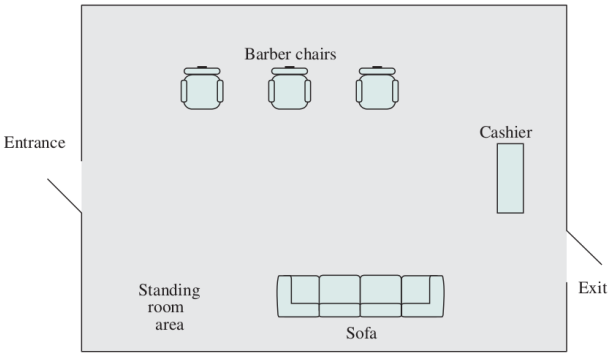
\includegraphics[width=0.6\linewidth]{images/negozio-barbiere.PNG}
        %\captionof{figure}{Esempio di semaforo}
    \end{minipage}

    Una delle migliori soluzione per questo problema è la seguente:
    \begin{lstlisting}[language=C]
    int next_barber;

    void Barber(i) {
        while(true) {
            wait(mutex);
            next_barber = i;
            signal(chair);
            wait(ready);
            signal(mutex);
            cut_hair();
            signal(finish[i]);
            wait(paym);
            accept_pay();
            signal(recpt);
        }
    }
    
    void Customer(){int my_barber;
        wait(max_cust);
        enter_shop();
        wait(sofa);
        sit_on_sofa();
        wait(chair);
        get_up_from_sofa();
        signal(sofa);
        my_barber = next_barber;
        sit_in_chair();
        signal(ready);
        wait(finish[my_barber]);
        leave_chair();
        pay();
        signal(paym);
        wait(recpt);
        exit_shop();
        signal(max_cust);
    }
    \end{lstlisting}
\end{Example}

\section{Mutua esclusione: soluzioni software}
Un altro modo per risolvere i problemi semplici di concorrenza è attraverso soluzioni software. 

\subsection*{Algoritmo di Dekker}
Una soluzione si può ottenere è con l'algoritmo di Dekker (vedi Figura \ref{fig:dekker}).

\begin{figure}[h]
    \centering
    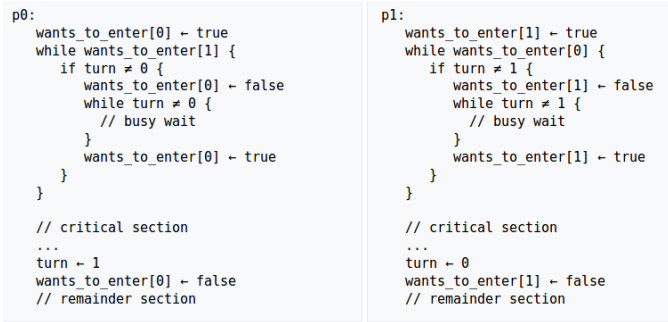
\includegraphics[width=0.9\linewidth]{images/dekker.PNG}
    \caption{Algoritmo di Dekker}
    \label{fig:dekker}
\end{figure}

Questo algoritmo vale solo per due processi con i flag inizializzati a 0 e \verb|turn| che può assumere 0 o 1. Grazie a questo garantisce la non-starvation e il non-deadlock, inoltre non richiede supporto dal sistema operativo.

\subsection*{Algoritmo di Peterson}
L'algoritmo di Peterson risolve il problema in maniera più semplice garantendo gli stessi vantaggi visti per l'algoritmo di Dekker (vedi Figura \ref{fig:Peterson}).

\begin{figure}[h]
    \centering
    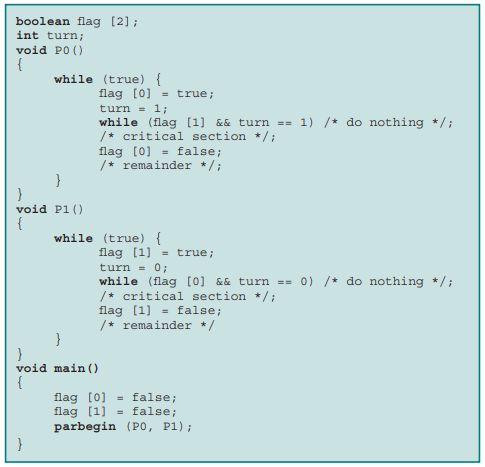
\includegraphics[width=0.6\linewidth]{images/Peterson.PNG}
    \caption{Algorimo di Peterson}
    \label{fig:Peterson}
\end{figure}

\section{Passaggio di messaggi}
Quando un processo interagisce con un altro, deve soddisfare due requisti: sincronizzazione (con la mutua esclusione) e la comunicazione. Lo scambio di messaggi (\textit{message passing}) è una soluzione alla comunicazione utilizzabile sia con memoria condivisa che distribuita. Le operazioni fondamentali per lo scambio di messaggi sono: mando il messaggio, \verb|send(destination, message)|, e ricevo il messaggio, \verb|receive(source, message)|; spesso, oltre a queste due, c'è il test di recezione che controlla solo se c'è un messaggio da ricevere. 

\subsection*{Sincronizzazione}
La comunicazione richiede anche la sincronizzazione, infatti, il mittente deve inviare prima che il ricevente riceva e sia mittente che destinatario possono essere bloccanti o non bloccanti:

\begin{itemize}
    \item con Send e Receive bloccanti, sia il mittente che il destinatario sono bloccati finché il messaggio non è completamente ricevuto (tipicamente viene chiamato \textit{rendezvous});

    \item con Send non bloccante (\verb|nbsend|) e Receive bloccante, il mittente non viene mai messo in blocked e continua con le sue operazioni e il destinatario rimane bloccato finché non ha ricevuto il messaggio;

    \item con Receive non bloccante (\verb|nbreceive|), se il messaggio è presente viene ricevuto, altrimenti si va avanti. Si utilizza un bit dentro il messaggio per dire se la recezione è avvenuta oppure no.
\end{itemize}

Tutte queste operazioni sono rese atomiche dal sistema operativo, ovvero un solo processo per volta le esegue finché non viene completata, oppure finché il processo non viene bloccato.

\subsection*{Indirizzamento}
Il mittente e il destinatario devono poter dire a quale processo (o quali processi) voler mandare/ricevere il messaggio. Per questo scopo si possono usare l'indirizzamento diretto oppure indiretto.

Con l'indirizzamento diretto l'operazione di send include uno specifico identificatore per il destinatario, o per un gruppo di destinatari. Si può utilizzare lo stesso approccio per la receive in modo da ricevere solo se il mittente coincide con il sender, oppure si può ricevere da chiunque. Ogni processo ha una sua coda, e una volta piena, solitamente il messaggio si perde o viene ritrasmesso.

Con l'indirizzamento indiretto i messaggi sono inviati ad una casella di posta (\textit{mailbox}) condivisa che viene esplicitamente creata da un qualche processo. Il mittente manda messaggi alla mailbox, da dove il destinatario se li va a prendere e se la ricezione è bloccante, e ci sono più processi in attesa su una ricezione, un solo processo viene svegliato.

\begin{figure}[h]
    \centering
    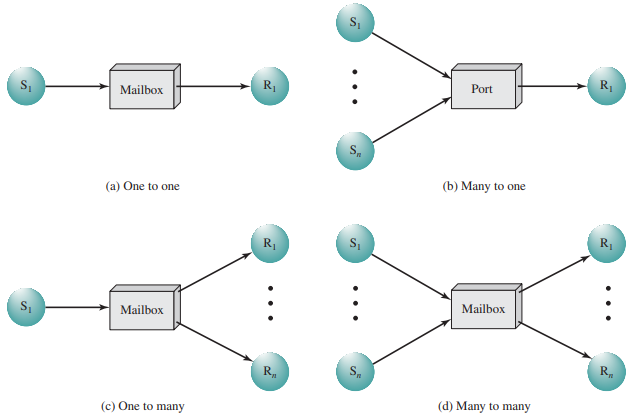
\includegraphics[width=0.65\linewidth]{images/tipi-di-comunicazione.PNG}
    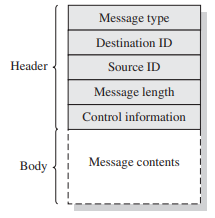
\includegraphics[width=0.29\linewidth]{images/formato-dei-messaggi.PNG}
    \caption{Tipi di comunicazione indiretta e formato dei messaggi}
    \label{fig:tipi-di-comunicazione}
\end{figure}

\subsection*{Mutua esclusione}
Possiamo utilizzare i messaggi per la mutua esclusione:
\begin{lstlisting}[language=C]
    const message null = /* null message */;
    mailbox box;
    void P(int i) {
        message msg;
        while(true) {
            receive(box, msg);
            /* critical section */;
            nbsend(box, msg) ;
            /* remainder */;
    } }

    void main() {
        box = create_mailbox() ;
        nbsend(box, null) ;
        parbegin(P(1), P(2), ..., P(n));
    }
\end{lstlisting}

Si può risolvere anche il problema del produttore/consumatore con i messaggi nel seguente modo:
\begin{lstlisting}[language=C]
    const int capacity = /* buffering capacity */ ;
    mailbox mayproduce, mayconsume ;
    const message null = /* null message */;
    
    void main ()
    {
        mayproduce = create_mailbox(),
        mayconsume = create_mailbox();
        for(int i=1; i<= capacity; i++)
            nbsend(mayproduce, null);
        parbegin(producer, consumer);
    }
    
    void producer() {
        message pmsg;
        while(true) {
            receive(mayproduce, pmsg);
            pmsg = produce();
            nbsend(mayconsume, pmsg);
        } }

    void consumer() {
        message cmsg;
        while(true) {
            receive(mayconsume, cmsg);
            consume(cmsg);
            nbsend(mayproduce, null);
    } }
\end{lstlisting}

\section{Problema dei lettori/scrittori}
Un problema che si può generare con la mutua esclusione è quello dei lettori/scrittori che nasce quando un'area dati è condivisa tra molti processi, dove alcuni la leggono e altri la scrivono. Le condizioni da soddisfare sono: più lettori possono leggere l'area contemporaneamente; solo uno scrittore può scrivere nell'area; se uno scrittore è all'opera sull'area, nessun lettore può effettuare letture. La differenza con il problema dei produttori/consumatori è che all'area condivisa si accede per intero, quindi si eliminano i problemi di buffer pieno o vuoto ma bisogna permettere ai lettori di accedere contemporaneamente. 

Una prima soluzione si può fare gestendo la priorità ai lettori o agli scrittori come mostrato in Figura \ref{fig:precendenza-lettori-scrittori}.

\begin{figure}[h]
    \centering
    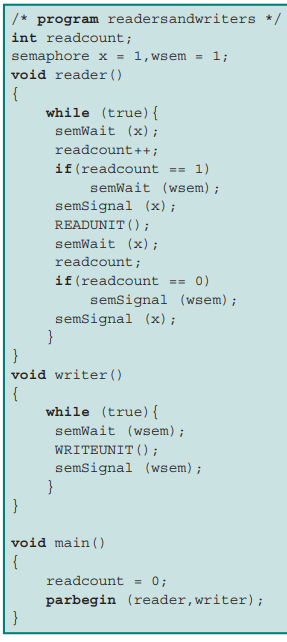
\includegraphics[width=0.44\linewidth]{images/precedenza-lettori.PNG}
    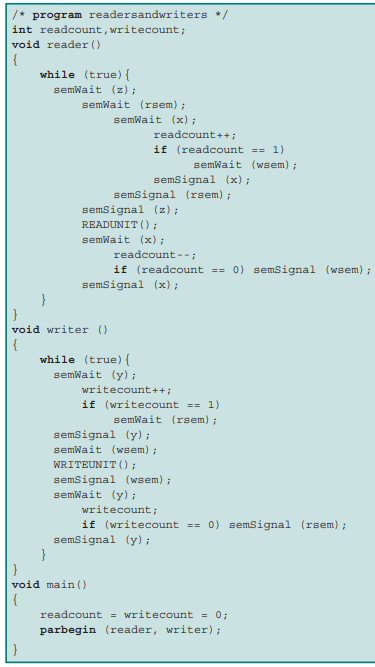
\includegraphics[width=0.55\linewidth]{images/precedenza-scrittori.PNG}
    \caption{Precedenza ai lettori e precedenza agli scrittori}
    \label{fig:precendenza-lettori-scrittori}
\end{figure}

E' possibile anche utilizzare i messaggi per risolvere il problema dei lettori/scrittori:
\begin{lstlisting}[language=C]
    void reader(int i)
    {
    while(true) {
        nbsend(readrequest, null);
        receive(controller_pid, null);
        READUNIT();
        nbsend(finished, null);
    } }

    void writer(int j)
    {
    while(true) {
        nbsend(writerequest, null);
        receive(controller_pid, null);
        WRITEUNIT();
        nbsend(finished, null);
    } }

    void controller () {
        int count = MAX_READERS;
        while(true) {
            if(count > 0) {
                if(!empty(finished)) { /* da reader ! */
                    receive(finished, msg);
                    count ++;
                }
                else if(!empty(writerequest)) {
                    receive(writerequest, msg);
                    writer_id = msg.sender;
                    count = count - MAX_READERS;
                }
                else if(!empty(readrequest)) {
                    receive(readrequest, msg);
                    count --;
                    nbsend(msg.sender, "OK");
            } }
            if(count == 0) {
                nbsend(writer_id, "OK");
                receive(finished, msg); /* da writer ! */
                count = MAX_READERS;
            }
            while(count < 0) {
                receive(finished, msg); /* da reader ! */
                count ++;
            } /* while (count < 0) */
        } /* while (true) */
    } /* controller */
\end{lstlisting}

\section{Equivalenze}
La condivisione di risorse può quindi essere implementata con tre metodi diversi: istruzioni hardware, sincronizzazione (semafori) e message passing. Se si può implementare un'applicazione con uno qualsiasi dei tre metodi, allora lo si può fare anche con gli altri due. Un particolare meccanismo potrà rivelarsi più conveniente degli altri, in termini di facilità di sviluppo, di prestazioni, e di gestione.